\documentclass[]{article}
\usepackage{graphicx}
\usepackage{hyperref}

\usepackage{color}
%\usepackage{listings}

\definecolor{light-gray}{gray}{0.60}
\newcommand{\cmt}[1]{ {\color{light-gray}\it/** #1 **/} }


\newcommand{\todo}[1]{\textcolor{red}{\textbf{TODO : #1}}}
\newcommand{\important}[1]{\textcolor{red}{/!\textbackslash} #1}

%opening
\title{Puck manual}
\author{}



\begin{document}

\maketitle

\begin{abstract}

\end{abstract}

\section{User Interface}

Puck's interface is composed of four panels(cf figure \ref{fig:screenshot}). 

\begin{figure}
	\centerline{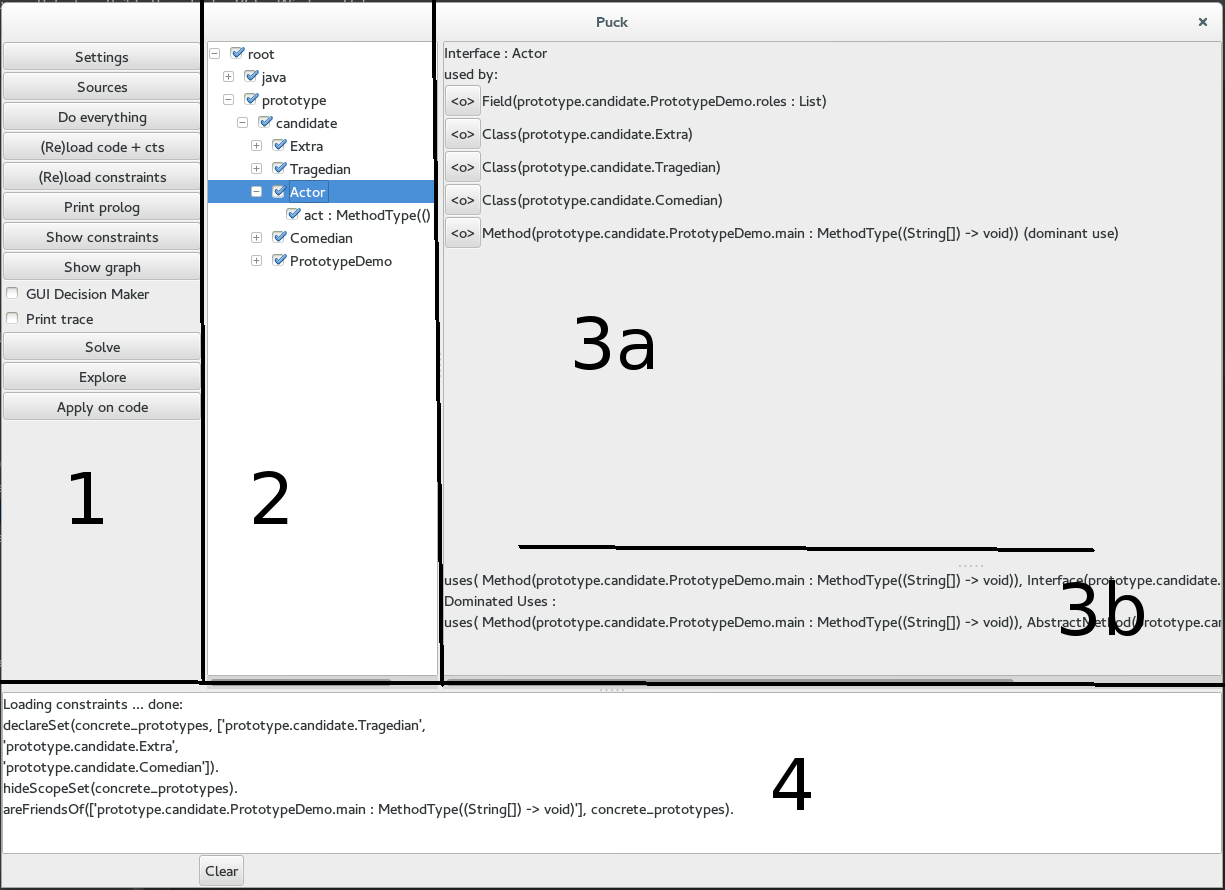
\includegraphics[keepaspectratio, width=1.7\textwidth]{screenshot.png}}
	\caption{Screen-shot of main panel of puck}
	\label{fig:screenshot}
\end{figure}

\begin{enumerate}
\item the button panel
\item the package explorer
\item the node information panel
\item the console
\end{enumerate}

Settings and global control is done in the button panel. Once an access graph is loaded, you can browse the different nodes in the package explorer. When you click on a node, detailed information are displayed on the node information panel. The console displays various informations. You can clear it at any time with the \verb|Clear| button. The button panel and the node information panel are detailed below.

\subsection{Button Panel}
\subsubsection{Simple use}

A normal work space for puck is composed by a folder containing java sources (1.4 or 1.5).
A file named \verb|decouple.pl| placed at the root of the work space.

Optionally the following input can also be given to puck by placing them at the root of the work space :
\begin{itemize}
\item \verb|jar.list| : A file containing a list of absolute paths to jar archives (one per line), if the sources requires external libraries to compile.
\item \verb|api_nodes| : A list of elements of the java standard library that you wish to see displayed on the graph.
\end{itemize} 

The most simple use case, if you have a work space containing the above mention files with the default name and path, you just have to select it with the
 \verb|Work space| button and press \verb|Dot it !|\footnote{puck takes the directory from where it was open as its default work space, so if you open puck from your work space root you just have to click Dot it !}.
 Puck will then 
 \begin{enumerate}
 	\item load the Java sources and create an access graph
 	\item load the coupling constraints
 	\item display the access graph with violations marked in red
 	\item solve the constraints with a default strategy
 	\item display the solved access graph
 	\item apply the computed change on the source code
 	\item open the original sources and the modified ones 	
 \end{enumerate}

\subsubsection{Buttons decsription}

\begin{itemize}
	\item \verb|Settings|\\
	Open a window when you can change the default values.\\
	\important{Puck relies on Graphviz dot\cite{graphviz} to generate the visual version of the graph. If it is not accessible from your PATH system variable, you need to set dot executable path in this setting window.}
	
	\item \verb|Work space|\\
	Let you choose a work space and try to load the source code.
	
	\item \verb|Do it !|\\
	Do the process describe above.
	
	\item \verb|(Re)load code & constraints|\\
	(Re)load the code from the current source path. If you edit your sources outside of puck, or if you open puck at the root directory of your sources files you can (re)load them with this button. It will also load the constraint file.
	
	\item \verb|(Re)load constraints|\\
	This will remove any loaded constraint on the graph and reload the constraint file. Useful while you are editing your constraint file.
	
	\item \verb|Print prolog|\\
	This print a prolog representation of the access graph.
	
	\item \verb|Show constraints|\\
	Print the loaded constraint in the console.
	
	\item \verb|Show graph|\\
	Display a graphic version of the access graph with constraint violations in red.
	
	\item \verb|GUI Decision Maker|\\
	Check this box to take the decision instead of the default strategy during the solving process.\\
	\todo{Finish implementation}
	
	\item \verb|Print trace|\\
	Check this box to create png files of the graph at each iteration of the solving process (work also for ``exploration'').
	
	\item \verb|Solve|\\
	Launch the solving process.
	
	\item \verb|Explore|\\
	Explore all choices during the solving process. Create png files of all the results. At the end of the process the graph state is the last one explored.
	\todo{Implement a menu to navigate between the solutions}
	
	\item \verb|Apply on code|\\
	Apply the changes computed to obtain the current code on the underlying representation of the code a reprint it in the output directory.
	
\end{itemize}

\subsection{Node information panel}
This screen is divided in two parts (cf 3a \& 3b on figure \ref{fig:screenshot}).
When you select a node in the package explorer, on the top of the node information panel, you can see the users of the selected node. If you click on the \verb|<o>| button next a user, it will display the graph with the uses (user, selected node) in bold, its dominant uses (if any) in blue and its dominated uses (if any) in green.
This information can also be accessed textually. The list of the dominant and dominated uses can be displayed at the bottom of the panel by clicking on the user node name.

\section{Constraint}
The parsed constraints have the following formal grammar:\footnote{facades, interlopers and friends are always scope sets}

\begin{itemize}
	\item $constraintFile$ \verb|::=(|$clause$\verb|)*| 
	
	\item \begin{tabbing}
		$clause$ \verb|::|\=\verb|=| java\_import($list$).\\		
		\>$|$ declareSet($ident$, $list$).\\
		\>$|$ declareSetUnion($ident$, $list$).\\
		\>$|\; constraint$
	\end{tabbing}
	\item \begin{tabbing}
		$constraint$ \verb|::|\=\verb|=| hideScope($ident$, $listOrIdent$, $listOrIdent$, $listOrIdent$).\\	
		\>\color{light-gray}{hideScope(scope, facades, interlopers, friends)}\\
		
		\>$|$ hideScopeSet($listOrIdent$, $listOrIdent$, $listOrIdent$, $listOrIdent$).\\
		\>\color{light-gray}{hideScopeSet(scopeSet, facades, interlopers, friends)}\\
		
		\>$|$ hideScopeSet($listOrIdent$).\\
		\>\color{light-gray}{hideScopeSet(scopeSet)}\\
			
		\>$|$ hideScopeSetFrom($listOrIdent$, $listOrIdent$).\\
		\>\color{light-gray}{hideScopeSetFrom(scopeSet, interlopers)}\\
			
		\>$|$ hideScopeFromEachOther($listOrIdent$).\\
		\>\color{light-gray}{hideScopeFromEachOther(scopeSet)}\\
		\\
		\>$|$ hide($ident$, $listOrIdent$, $listOrIdent$).\\
		\>\color{light-gray}{hide(element, interlopers, friends)}\\
		
		\>$|$ hideSet($listOrIdent$, $listOrIdent$, $listOrIdent$).\\	
		\>\color{light-gray}{hideSet(elementSet, interlopers, friends)}\\
		
		\>$|$ hideFrom($ident$, $listOrIdent$).\\	
		\>\color{light-gray}{hideFrom(element, interlopers)}\\
				
		\>$|$ hideSetFrom($listOrIdent$, $listOrIdent$).\\	
		\>\color{light-gray}{hideSetFrom(elementSet, interlopers)}\\
		\\
		
		\>$|$ isFriendOf($listOrIdent$, $listOrIdent$).\\
		\>\color{light-gray}{isFriendOf(scopeSet, beFriended)}\\
		
	\end{tabbing}

	\item \begin{tabbing}
		$ident$ \verb|::|\=\verb|=[^|[]',().\verb|]+|\\		
		\>$|$ '\verb|[^|'\verb|]+|'
	\end{tabbing}
	
	\item $list$ \verb|::=| [ ] $|$ [$ident$\verb|(|,$ident$\verb|)*|]\\		
	
	\item $listOrIdent$ \verb|::=| $list\; |\; ident$\\		
		
\end{itemize}


\section{Puck's Architecture}
Puck is written in scala. It's architecture is composed of the following packages: 
\begin{itemize}
\item \verb|puck|\\
	It is the root package, it contains only the Front object

\item \verb|puck.graph|\\
	This package and its subpackages contains the generic elements of the access graph. A lot of classes including AccessGraph and AGNode are parameterized by the node kind. This package contains mainly the classes describing the structure of the graph and its node.

\item \verb|puck.graph.backTrack|\\
	Even if scala promote the functional paradigm, the main purpose of puck is to compute modification on potential huge access graph. For this reason, AccessGraph and AGNode are mutable structure. This package contains what is necessary to undo/redo modification applied on the access graph.

\item \verb|puck.graph.constraints|\\
	It is here that we find the classes that relate to the constraints. It goes from the parser to the solver.

\item \verb|puck.graph.io|\\
	To graph printer are here. We also find here the FilesHandler : this class give some high level interface about the graph processing.

\item \verb|puck.gui|\\
	This package gather together the puck's graphical interface. As in \verb|puck.graph| the classes found here are generic and deals with generic AccessGraph.
	
\item \verb|puck.gui.decisionsFrames|\\
	This sub-package contains the different panel that let the user make its decisions when the constraint solving process offers several possibility.
	
\item \verb|puck.javaAG|\\
	All java specific material is gathered here. 
	In particular we find the AG2AST object that apply on the AST the transformations computed on the access graph.

\item \verb|puck.javaAG.nodeKind|\\
	This package contains the java node kind. Some language specific consideration about graph transformations are black boxed here.

\item \verb|puck.search|\\
	Contains a generic search engine framework. It is used both in the constraint solving process and in the graph transformation recording comparator.

\item \verb|puck.util|\\
This package contains 
\begin{itemize}
\item a generic breadth first iterator for trees
\item a mini logger framework
\item some basic file helper functions and a timer
\end{itemize}
\end{itemize}


\section{Solver built-in strategy}
The solver trait (\verb|puck.graph.constraints.Solver|) uses a decision maker. A decision maker is an interface that abstract how decision are made. Three implementations can be found in puck:
\begin{itemize}
	\item \verb|puck.graph.constraints.DefaultDecisionMaker|\\
	This decision maker make decisions based on a heuristic that will be explained in section.
	\item \verb|puck.gui.GUIDecisionMaker|\\
	This implementation uses windows to ask the user which decision to make. \todo{Implementation to finish}
	\item \verb|puck.graph.constraints.ConstraintSolvingSearchEngine|
	This implementation is based on the search engine. At a decision point it compute all the possible solutions. All choices can be explored thanks to backtrack.
\end{itemize}

However some decisions are hard coded. Some are imposed by the fact that the solving process is done on an access graph and we rely on the available information.
Other are the product of a heuristic to reduce the search state space. This choices are what is called the built-in strategy and explained here:

The main loop of the solver has the following instructions. It search for violations target, then try to solve as many of the violations with the same target as possible. Then it loop and do it again until there is no more violation.\\

The decision of the violation target is delegated to the decision maker.

To remove a uses violation we redirect it toward an abstraction of the target, in general a super type. Redirecting the source of use arc in term of code means doing an extract method. This refactoring is not computable on the access graph since to do it properly we need precise information about the context in which a element is used. The access graph does not give such informations.

To remove a contains violation, we move the target into another host, newly created if needed.

For a given violations target $t$, if it is wrongly contained, meaning that contains(\_, $t$) is a violations, we solve it before the uses violations.
If we solve the uses violations first, however $t$ is abstracted it won't change $t$ container and this contains violation will still have to be solved.
While when choosing a new host for $t$, we can find a host such that is also solves uses violations, thus preventing the creation of an uneeded abstraction that would complicate the software architecture.





\subsection{Hard coded choices}
\begin{itemize}
	\item for a given violations target, we solve the contain violation before the uses
	\item the uses violations are solved by abstracting the target
\end{itemize}


\section{DefaultDecisionMaker : explanation of the heuristic }




\bibliographystyle{abbrv}
\bibliography{manual}

\end{document}
